\documentclass{beamer}
\usepackage{subfig}
\usepackage{amsmath}
\usepackage{bm}

\DeclareMathOperator*{\argmax}{arg\,max}
\DeclareMathOperator*{\argmin}{arg\,min}


\title{Logistic Regression}
\author{Prof. Alessandro Lucantonio}
\institute{Aarhus University - Department of Mechanical and Production Engineering}
\date{?/?/2023}

\begin{document}
	\frame{\titlepage}
	
	\begin{frame}
		\frametitle{Binary classification}
		Classification : discrete target (output vector).
		
		Binary classification: $\{0,1\}$ target
		
		\vspace{5mm}
		Example of binary classification task: Spam/not spam emails.
		
		\vspace{5mm}
		Idea: consider hypothesis $h_w$ such that
		\begin{equation*}
			0 \leq h_{\bm{w}} \leq 1.
		\end{equation*}

		\begin{itemize}
			\item if $h_{\bm{w}}(\bm{x}) \geq 0.5$, predict $1$;
			\item if $h_{\bm{w}}(\bm{x}) < 0.5$, predict $0$.
		\end{itemize}
	\end{frame}

	\begin{frame}
		\frametitle{Logistic Regression}
		Hypothesis: $h_{\bm{w}}(\bm{x}) = \sigma(\bm{w}^T\bm{x})$, where
		\begin{equation*}
			\sigma(t) = \frac{1}{1+e^{-t}}
		\end{equation*}
		is the \textbf{sigmoid function}.
		
		\begin{figure}
			\centering
			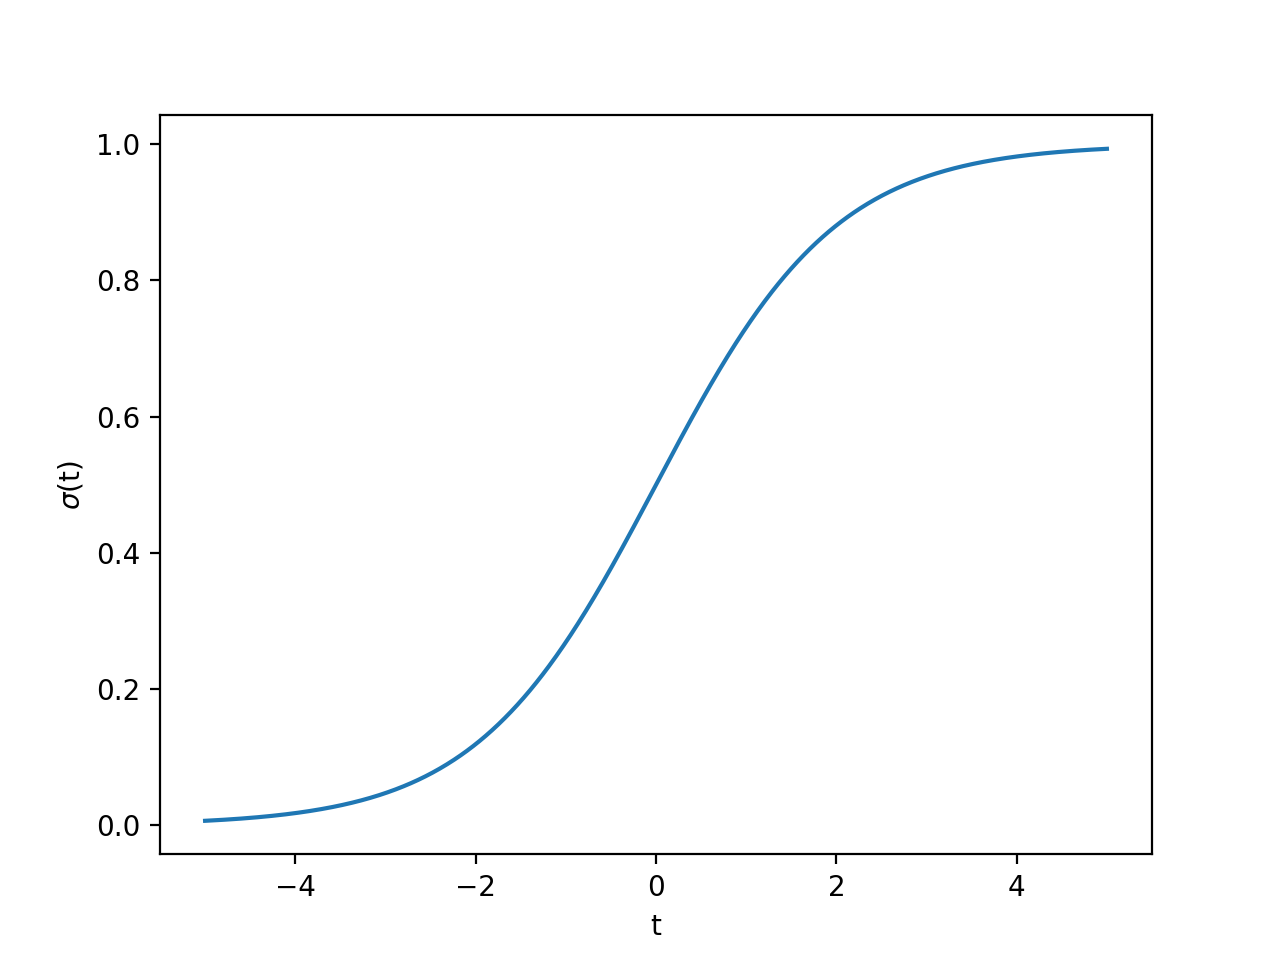
\includegraphics[scale=0.45]{images/sigmoid}
			\caption{Sigmoid function}
		\end{figure}
		
	\end{frame}

	\begin{frame}
		\frametitle{Decision boundary}
		\begin{figure}
			\centering
			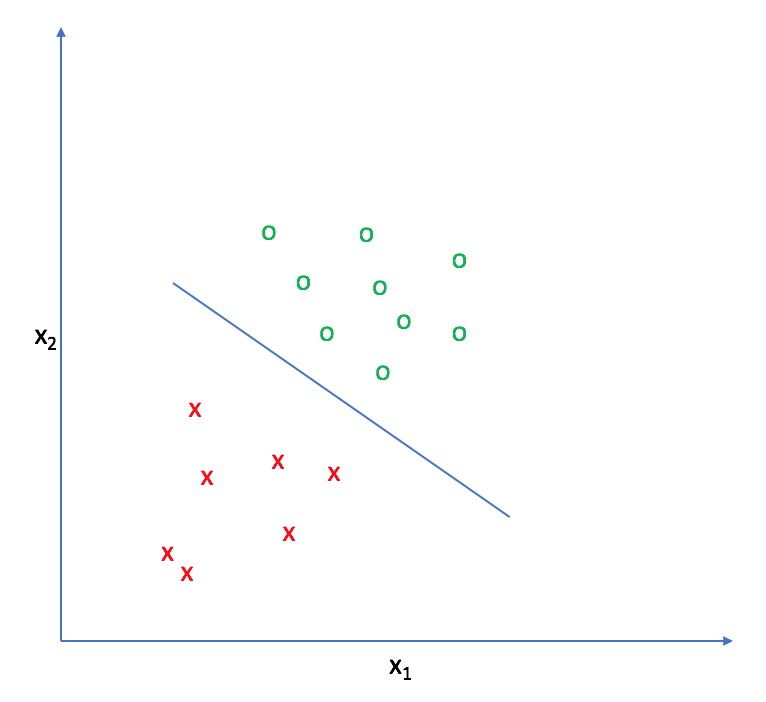
\includegraphics[scale=0.5]{images/decision_boundary}
			\caption{Trivial example of decision boundary}
		\end{figure}
	\end{frame}

	\begin{frame}
		content...
	\end{frame}
\end{document}